\documentclass{resume} % Use the custom resume.cls style



\usepackage[square,sort,comma,numbers]{natbib} % refer to https://tex.stackexchange.com/questions/54480/package-natbib-error-bibliography-not-compatible-with-author-year-citations to resolve the error...
\usepackage{bibentry}
\usepackage{multicol}  % 提供多栏环境
\usepackage{graphicx}

\usepackage[left=0.4 in,top=0.4in,right=0.4 in,bottom=0.4in]{geometry} % Document margins
\newcommand{\tab}[1]{\hspace{.2667\textwidth}\rlap{#1}} 
\newcommand{\itab}[1]{\hspace{0em}\rlap{#1}}
\name{Junyan Su} % Your name
% You can merge both of these into a single line, if you do not have a website.
%\address{+1(123) 456-7890 \\ San Francisco, CA} 
\address{Email: \href{mailto:junyan.su@my.cityu.edu.hk}{junyan.su@my.cityu.edu.hk} }
% \\ \href{https://linkedin.com/in/linkedinURL}{linkedin.com/in/linkedinURL}   %
\address{Homepage: \href{https://sujunyan.github.io}{sujunyan.github.io}}


% \usepackage[backend=bibtex]{biblatex}
% \addbibresource{\jobname.bib}
\begin{document}

\bibliographystyle{abbrv1}
\nobibliography{../../../_bibliography/underreview, ../../../_bibliography/papers}
% \nobibliography{../../../_bibliography/papers.bib}

%----------------------------------------------------------------------------------------
%----------------------------------------------------------------------------------------
%	EDUCATION SECTION
%----------------------------------------------------------------------------------------


\begin{rSection}{Education}

{Ph.D. in Data Science}, City University of Hong Kong  \hfill {2020-2025}\\
{B.E. in Computer Science and Technology}, ShanghaiTech University \hfill {2015-2019}

\end{rSection}

\begin{rSection}{Research Interests}
    My research interests are intelligent transportation systems, from the perspective of control and optimization. I also have broad interests in computing methods for energy systems.
\end{rSection}

\def\FormatName#1{%
    \def\myname{Junyan Su}%
    \edef\name{#1}%
    \ifx\name\myname
      \underline{#1}%
    \else
       #1%
    \fi
}

\begin{rSection}{Journal Articles}
    % $^*:$ Co-primary author. 
    \begin{enumerate}
        % \item \bibentry{su2025optimizing}.
        \item \underline{Junyan Su}, Qiulin Lin, and Minghua Chen. Optimizing Carbon Footprint in Long-Haul Heavy-Duty E-Truck Transportation. \textcolor{blue}{\textit{Nature Communications}}, accepted for publication, 2025. 
        \item \bibentry{lin2025optimala}.
        \item \bibentry{jiang2025fast}.
        \item \bibentry{su2024minimizing}.
        \item \bibentry{jiang2020distributed}.
    \end{enumerate}
\end{rSection}

\begin{rSection}{Conference Papers}
    % \bibliographystyle{mybibstyle}
    %% Refer to the following link to highlight my own name.
    %% https://tex.stackexchange.com/questions/33330/make-one-authors-name-bold-every-time-it-shows-up-in-the-bibliography/33379#33379
    
    % \nobibliography{papers.bib}
    \begin{enumerate}
         \item \bibentry{lin2024competitive}.
         \item \bibentry{su2023minimize}.
         \item \bibentry{su2023follow}. \textcolor{blue}{Best Paper Award}.
    % \begin{enumerate}
    %     \item \bibentry{su2023follow} \textbf{(Best Paper Award)}
    %     \item \bibentry{jiang2020distributed}
    % \end{enumerate}
    % \textbf{Other Publication:}
        \item \bibentry{lin2022competitive}.
        % \item \bibentry{su2022e2pilot}.
        % \item \bibentry{su2021energy}.
        \item \bibentry{su2020distributed}.
        \item \bibentry{gao2020efficient}.
        % \item \bibentry{su2019interval}.
    \end{enumerate}
\end{rSection}

% \begin{rSection}{Working Papers}
%     \begin{enumerate}
%          \item \bibentry{su2025maximizing}.
%          \item \bibentry{lin2025optimal}.
%     \end{enumerate}
%          % \item \bibentry{su2025maximizing}.
% \end{rSection}


\newpage

\begin{rSection}{Award and Recogition}
    % \begin{multicols}{1}
    % \begin{itemize}
        \textbf{Academic Awards:}
        \begin{itemize}
            \item Outstanding Academic Performance Award, City University of Hong Kong, 2023
            \item ACM e-Energy Best Paper Award, 2023
        \end{itemize}
        
        \textbf{Competition Awards:} 
        \begin{itemize}
            \item Second Place, Meituan UAV Competition, 2023
        \end{itemize}
        
        \textbf{Entrepreneurship Grants:} 
        \begin{itemize}
            \item HK Tech 300 \& HKTSP Seed Fund, 2022
        \end{itemize}
        
        \textbf{Scholarships and Student Awards:}
        \begin{itemize}
            \item CDC Student Travel Grant \& Workshop Support, 2023
            \item Research Tuition Scholarship, City University of Hong Kong, 2023
            \item Outstanding Graduate Award, ShanghaiTech University, 2019
        \end{itemize}
    % \end{itemize}
    % \end{multicols}
    
    % Outstanding Student, ShanghaiTech University, 2016,2017,2018.
\end{rSection}

\begin{rSection}{Software \& Skills}
    \begin{itemize}
        \item 
        \begin{minipage}[h]{0.64\textwidth} % 左边文字部分,占60%宽度
            \textbf{Main developer} of the \href{https://www.e2pilots.com/}{\textcolor{blue}{E2Pilot}}, a navigation platform for energy-efficient long-haul timely truck transportation. The system contains a website interface and a mobile app interface. Given the origin, destination, and the deadline by the user, our system will compute the energy-efficient path and speed plan, as well as intelligent driving instructions to help truckers save the energy cost while delivering the goods on time. 
        \end{minipage}%
        \hfill % 在左右两部分之间添加间距
        \begin{minipage}[h]{0.32\textwidth} % 右边图片部分,占35%宽度
            \centering
            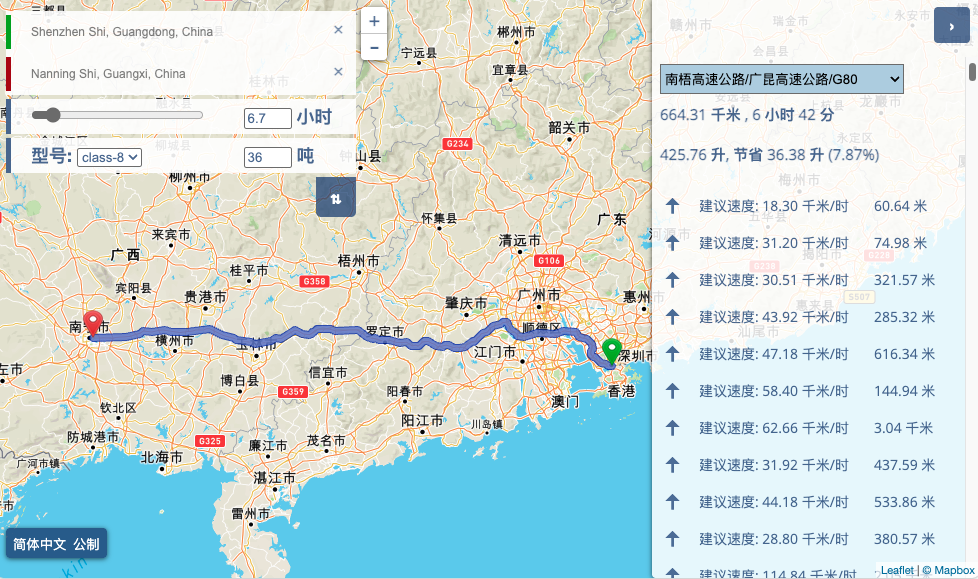
\includegraphics[width=.80\textwidth]{e2pilot-web.png} % 替换为你的图片路径
            % \captionof{figure}{E2Pilot 系统界面} % 可选的图片标题
        \end{minipage}

        \item \textbf{Main developer} of the \href{https://github.com/sujunyan/ParExMPC}{\textcolor{blue}{ParExMPC}}, an open-source toolbox for real-time close-to-optimal Model Predictive Control (MPC) design providing MATLAB-based user interface and tailored C-code solver. The user could define the MPC problem with the MATLAB interface and generate the C-code that can be easily deployed resource-constrained embedded systems.
        \item \textbf{Main contributor} of the simulation for ALL the publication I co-authored. 
        \item \textbf{Programming languages:} working knowledge of Julia, Python, C/C++, MATLAB.
    \end{itemize}
\end{rSection}

% \newpage

\begin{rSection}{Presentations}
    \begin{itemize}
        \item ``E2Pilot: A Navigation Platform for Energy-Efficient Timely Transportation of Long-Haul Heavy-Duty Trucks'', Prototypes for Humanity, Dubai, November 2024.
        \item ``Minimizing Carbon Footprint for Timely E-Truck Transportation: Hardness and Approximation Algorithm'', 
        CDC 2023, Singpore, December 2023.
        \item ``Follow the Sun and Go with the Wind: Carbon Footprint Optimized Timely E-Truck Transportation'', ACM e-Energy 2023, Orlando, Florida, June 2023.
    \end{itemize}
\end{rSection}

\begin{rSection}{Patents}
    \begin{itemize}
        \item M. Chen., \underline{J. Su}, and Q. Lin, ``Carbon Footprint Optimized Timely E-Truck Transportation", 14 Aug 2025, U.S. Patent No. US2025/0258006.
        % \item M. Chen., \underline{J. Su}, and Q. Lin, ``Carbon Footprint Optimized Timely E-Truck Transportation", 8 Feb 2024, (Filed) U.S. Patent Application No. 18/436,350.

        % Carbon Footprint Optimized Timely E-Truck Transportation CHEN, M., SU, J. & LIN, Q., 8 Feb 2024, (Filed) Priority No. 18/436,350 Research output: Patents, Agreements and Assignments › RGC 51 - Patents (CityU)
    \end{itemize}
\end{rSection}


%----------------------------------------------------------------------------------------
% TECHINICAL STRENGTHS	
%----------------------------------------------------------------------------------------
% \begin{rSection}{SKILLS}
% \begin{tabular}{ @{} >{\bfseries}l @{\hspace{6ex}} l }
% Progamming Languages & Julia, Python, C/C++, MATLAB \\
% % Frameworks & React, Redux, Node.js, Express, Django, Mocha \\
% % Tools & Git, Docker, TravisCI, Kubernetes, AWS\\
% % Soft Skills & Time Management, Teamwork, Communication, Problem Solving, Leadership, Accountability
% \end{tabular}\\
% \end{rSection}


%----------------------------------------------------------------------------------------
% Projects
%----------------------------------------------------------------------------------------
%\begin{rSection}{PROJECTS}
%\vspace{-1.25em}
%\item \textbf{Project 1} {Language 1, Framework 1, Database, Language 2, Framework 2, DevOps Tooling} \hfill \href{www.github.com/GITHUBURL}{GitHub}
%\begin{itemize}
%    \itemsep -3pt {} 
%     \item Created a XYZ feature to accomplish ABC.
%     \item Retrieved data from XYZ to for ABC.
%    \item Implemented XYZ library for ABC.
%    \item Utilized XYZ that increased A by B\%.
% \end{itemize}
%\item \textbf{Project 2} {Language 1, Framework 1, Database, Language 2, Framework 2, DevOps Tooling} \hfill \href{www.github.com/GITHUBURL}{GitHub}
%\begin{itemize}
%    \itemsep -3pt {} 
%     \item Created a XYZ feature to accomplish ABC.
%     \item Retrieved data from XYZ to for ABC.
%    \item Implemented XYZ library for ABC.
%    \item Utilized XYZ that increased A by B\%.
% \end{itemize}
%\item \textbf{Project 3} {Language 1, Framework 1, Database, Language 2, Framework 2, DevOps Tooling} \hfill \href{www.github.com/GITHUBURL}{GitHub}
%\begin{itemize}
%    \itemsep -3pt {} 
%     \item Created a XYZ feature to accomplish ABC.
%     \item Retrieved data from XYZ to for ABC.
%    \item Implemented XYZ library for ABC.
%    \item Utilized XYZ that increased A by B\%.
% \end{itemize}
%\end{rSection} 

%----------------------------------------------------------------------------------------
% \begin{rSection}{Extra-Curricular Activities} 
% \begin{itemize}
%     \item 	Sample bullet point.
%     \item	Sample bullet point.
% \end{itemize}
% 
% 
% \end{rSection}

%------------------------
% Use this more detailed section if you have Relevant work experience
% keep your resume to 1 page, if you need to remove a project to display relevant experience
% that is okay
% ----------------------------
% \begin{rSection}{EXPERIENCE}

% \textbf{Role Name} \hfill Jan 2017 - Jan 2019\\
% Company Name \hfill \textit{San Francisco, CA}
%  \begin{itemize}
%     \itemsep -3pt {} 
%      \item Achieved X\% growth for XYZ using A, B, and C skills.
%      \item Led XYZ which led to X\% of improvement in ABC
%     \item Developed XYZ that did A, B, and C using X, Y, and Z. 
%  \end{itemize}
 
% \textbf{Role Name} \hfill Jan 2017 - Jan 2019\\
% Company Name \hfill \textit{San Francisco, CA}
%  \begin{itemize}
%     \itemsep -3pt {} 
%      \item Achieved X\% growth for XYZ using A, B, and C skills.
%      \item Led XYZ which led to X\% of improvement in ABC
%     \item Developed XYZ that did A, B, and C using X, Y, and Z. 
%  \end{itemize}

% \end{rSection} 

%\begin{rSection}{Work History}
%\vspace{-1.25em}
%\item \textbf{Job Title} {Company} \hfill Month Year - Month Year
%\item \textbf{Job Title} {Company} \hfill Month Year - Month Year
%\item \textbf{Job Title} {Company} \hfill Month Year - Month Year
%\end{rSection} 

%----------------------------------------------------------------------------------------

\end{document}